%
% ---------------------------------------------------
%
% Proyecto de Final de Carrera:
% Author: Alejandro Hernández Padrón <alu0100703511@ull.edu.es>
% Capítulo: Objetivos 
% Fichero: Cap1_Goals.tex
%
% ----------------------------------------------------
%

\chapter{RA en entornos universitarios } \label{chap:RAEntornosUniversitarios}  

En este capítulo se expondrán los usos y ventajas de la integración de la realidad aumentada en entornos universitarios.

La realidad aumentada se presenta en el ámbito educativo como una tecnología capaz de aportar transformaciones significativas a la forma en que el alumnado percibe y accede a la realidad física, proporcionando así, experiencias de aprendizaje más ricas e inmersivas.

En la actualidad en educación, la realidad aumentada rara vez se usa, pero cada vez más docentes, investigadores y desarrolladores están comenzando a moverse hacia nuevos métodos de enseñanza más interactivos. Por ello, la continua implantación de nuevas tecnologías en las aulas, junto al incremento de dispositivos móviles en la población, sitúa a la RA en una posición destacada para introducirse en las aulas. 

Las aplicaciones que tiene la RA, en lo referente a la creación de materiales didácticos y actividades de aprendizaje son múltiples, directas y fáciles de imaginar en prácticamente todas las disciplinas, sobre todo, las relacionadas con las ciencias aplicadas (ingeniería, química y física, biología), pero también en el campo del diseño industrial, la cirugía, la arqueología, etc.
La tecnología de la RA permite cambiar la forma de entender los contenidos de aprendizaje, puesto que aporta nuevas formas de interacción con el mundo real a través de capas digitales de información que amplían, completan y transforman en cierto modo la información inicial.

Los beneficios potenciales de la RA aplicados a la educación incluyen:
\begin{itemize}

    \item Aumentar o enriquecer la información de la realidad para hacerla más comprensible al alumno.
    
    % \item Permite múltiples formas de visualización de conceptos teóricos difíciles.

    \item El uso de una interfaz tangible para la manipulación de objetos, que permite observar un objeto desde diferentes puntos de vista,
    seleccionando, el discente, el momento y posición de observación.

    \item Potenciar el aprendizaje ubicuo \cite{URL::AprendizajeUbicuo}.
    
    \item Crear escenarios ``artificiales'' seguros para el alumnado
    como pueden ser laboratorios o simuladores. 

    \item Enriquecer los materiales impresos para el alumnado con información adicional en diferentes soportes.
    
    \item Facilita la colaboración efectiva y discusión entre el alumnado.
    
\end{itemize}

Numerosos trabajos han demostrado la eficacia de que las aplicaciones de RA pueden mejorar el proceso de aprendizaje, aumentar la motivación y la efectividad \cite{URL::animationeco} \cite{URL::ar2}. 

A la hora de diseñar un sistema de RA orientado a la enseñanza, existen una serie de requisitos para que el alumno no se distraiga con su uso y asegurar que el objetivo de mejorar el aprendizaje se cumpla. Los requisitos de estos sistemas de RA son:

\begin{itemize}
    \item Ser sencillo y robusto.
    \item Permitir que el educador ingrese información de manera simple y efectiva.
    \item Proporcionar al alumno información clara y concisa.
    \item Permitir una fácil interacción entre estudiantes y educadores.
    \item Realizar procedimientos complejos transparentes para los alumnos.
    \item Ser rentable y fácilmente extensible.
\end{itemize}

\section{Aplicaciones en entornos universitarios}

Las aplicaciones de la RA en entornos universitarios son múltiples y diversas y no solo se encuentran enfocadas al ámbito de la enseñanza. 
A continuación, analizaremos las posibles aplicaciones que se encuentran de la tecnología de RA en la actualidad para el colectivo universitario.

\subsection{Prácticas en laboratorios} 
En las realizaciones de las prácticas en un laboratorio, existe una gran gama de herramientas y máquinas que son desconocidas para el alumno. Para facilitar el uso de este instrumental, la RA permite asociar a cada elemento del laboratorio, información sobre el mismo, tutoriales de uso, indicaciones de los pasos a seguir para la elaboración de la práctica. 
Esto permite agilizar el proceso de realización de las prácticas evitando que el alumnado requiera del profesorado para resolver parte de sus dudas y permitiéndole centrarse más en la realización de la práctica.

\subsection{Practicas de campo y visitas} 

La posibilidad de realizar una visita a un museo e identificar cada estatua o cuadro, y mostrar información adicional sobre su autor, datos históricos sobre las obras artísticas, reconocer estilos e influencias del autor para su realización, permite al usuario mejorar su adquisición de conocimiento al mezclarse el objeto de información y conocimiento acerca de aquél en el mismo lugar. 
Este mismo concepto se puede aplicar a prácticas de campo a medios rurales, bosques, montañas y lagos, permitiendo al usuario identificar la flora y la fauna del terreno y mostrar características únicas sobre ellos, que a simple vista son imperceptibles. 
 
\subsection{Libros y documentos}

La RA permite el enriquecimiento de los textos de libros y documentos con información adicional referente al tema tratado en la lectura. Esta información puede ser un vídeo, texto adicional con información específica, un enlace web o incluso una representación en 3D de un objeto, con el que alumno pueda interactuar, con una explicación detallada del contenido teórico que se muestra en el libro. Esto promueve diferentes formas de asimilar el contenido de los libros con métodos más interactivos y participativos, lo cual mejora el proceso de aprendizaje.

\subsection{Aprendizajes experimentales} 

Cada área o disciplina que se imparte en cualquier tipo de formación o titulación universitaria consta de parte experimental. A la realización de esta parte experimental se le pueden aplicar técnicas de RA que faciliten el aprendizaje y el desarrollo de competencias transversales. Un ejemplo del uso de la RA, se puede encontrar en medicina donde el uso de visores como las Google Glass pueden ayudar a la alumna a identificar anatómicamente las partes del cuerpo de un paciente al que se le está realizando una operación en el quirófano. 
En disciplinas de ingeniería o arquitectura la integración de técnicas de RA permite la visualización de modelos 3D de edificios y construcciones.

\subsection{Información sobre la universidad}  

Dentro de las aplicaciones de la RA a los centros referidos al ámbito universitario, se encuentra el uso de marcadores y de técnicas de localización para dotar al alumno de información sobre: eventos, seminarios, jornadas culturales y guiar al usuario hasta la ubicación, recinto, aula o sala en la que se desarrollan estas actividades. También permite a los usuarios inscribirse de manera simple y cómoda a estos eventos, con el simple escaneo de un código QR asociado.

Este ámbito de utilización de la RA en entornos universitarios es el que se ha elegido como caso de uso para
el desarrollo de \ULLAR{}.

\section{Ejemplos de uso de la RA}

A continuación se comentarán algunas de las aplicaciones de técnicas de RA que se pueden encontrar en la actualidad.

% En la actualidad ya podemos encontrar aplicaciones funcionales de la tecnología de la RA. XXX

\subsection{Fabricación de un automóvil de carreras} 

El alumnado de la Universidad de Bath está utilizando una nueva herramienta RA desarrollada por la compañía de tecnología Rocketmakers. 
La herramienta RA ayudará en la construcción de la carcasa del automóvil, conocida como monocasco, específicamente con la aplicación de laminados de fibra de carbono. 
Su vehículo competirá en la competición de Fórmula Estudiantil 2019 organizada por la Institución de Ingenieros Mecánicos.

\begin{figure}[h]
    \centering
    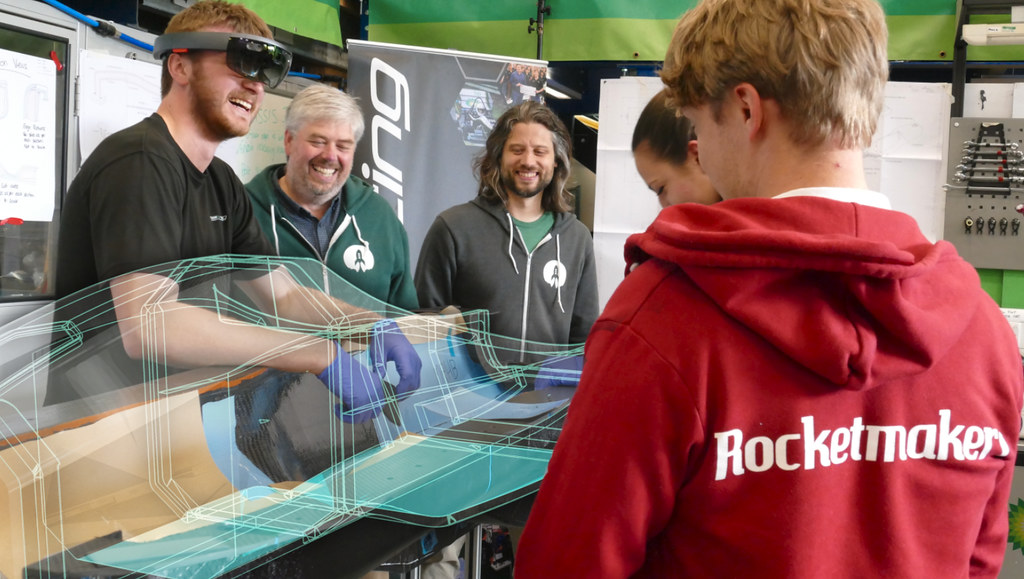
\includegraphics[width=0.6\linewidth]{carAR}
    \caption{Construcción de un automóvil de carreras gracias a la RA.}
    \label{fig:xyz}
\end{figure}    

Este proceso se llevará a cabo durante una semana, y los alumnos de Team Bath Racing trabajarán por turnos para aplicar cada laminado de fibra de carbono recortado en la ubicación correcta. La herramienta de Rocketmakers crea una versión RA del monocasco con la forma, ubicación y orientación correctas de cada segmento de laminado visible para el usuario durante el proceso de aplicación. Para ello utilizarán las Microsoft HoloLens \cite{URL::hololens}, con archivos de diseño asistido por computadora (CAD) que los alumnos han desarrollado.

 

\subsection{AR Sandbox} 
AR Sandbox \cite{URL::sandbox} es el resultado de un proyecto desarrollado por 
el \textit{UC Davis W.M. Keck Center for Active Visualization in the Earth Sciences} (KeckCAVES), 
conjuntamente con el \textit{UC Davis Tahoe Environmental Research Center}, el Lawrence Hall of Science, y el \textit{ECHO Lake Aquarium and Science Center}

El proyecto combina aplicaciones de visualización 3D con una exhibición de AR Sandbox para enseñar conceptos de ciencias de la tierra. 
El entorno de RA permite a los usuarios crear modelos de topografía al dar forma a la arena real, que luego se aumenta en tiempo real mediante un mapa de color de elevación, líneas de contorno topográficas y agua simulada. 
El sistema enseña conceptos geográficos, geológicos e hidrológicos, como la forma de leer un mapa topográfico, el significado de las curvas de nivel, las cuencas hidrográficas, los diques, etc.

\begin{figure}[h]
    \centering
    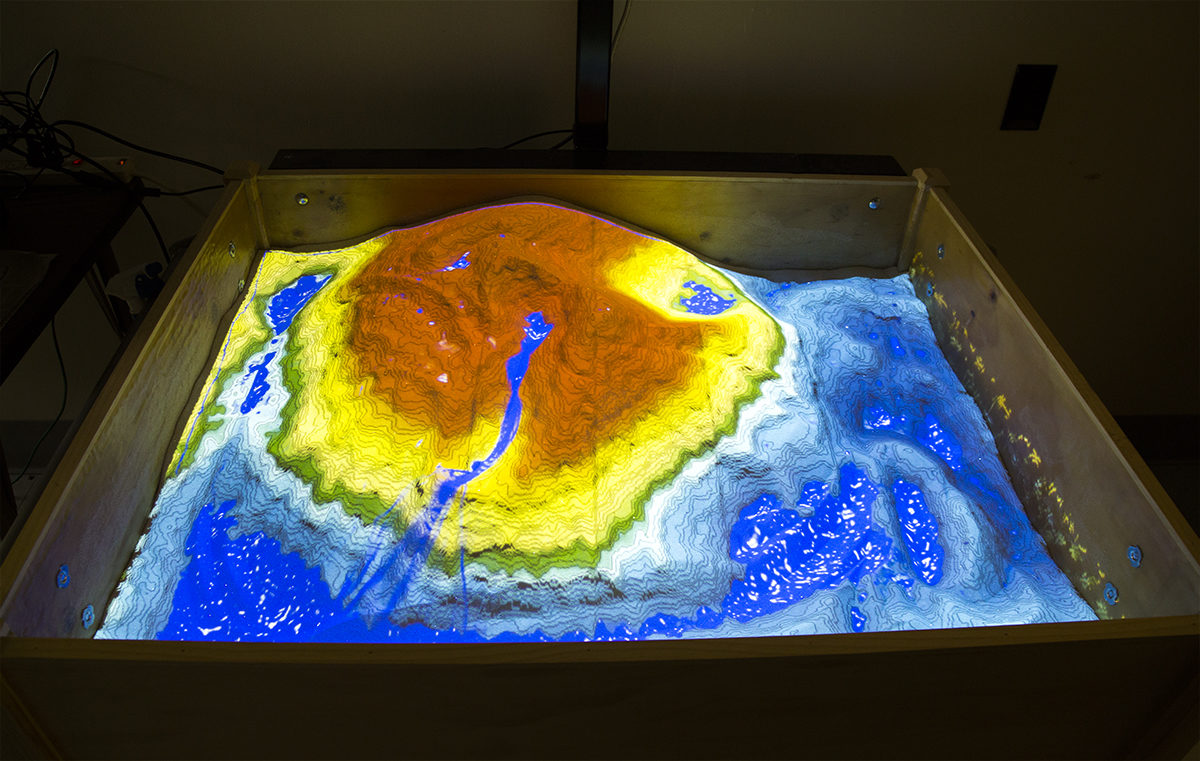
\includegraphics[width=0.8\linewidth]{sandAR}
    \caption{Funcionamiento de AR Sandbox.}
    \label{fig:xyz}
\end{figure}    







